\noindent Recall the propagator, or transition amplitude, for a nonrelativistic quantum system

\begin{equation}
U(q_i, q_f; T) = \left( \prod_j \int \mathcal{D} q^j (t) \int \mathcal{D} p^j (t) \right) e^{i \int^T_0 dt \, \mathcal{L} (q^j, \dot{q}^j)}.
\end{equation}

\noindent To work with this, we often discretize $q(t) \rightarrow q^j_k$

\begin{figure}[H]
	\centering
	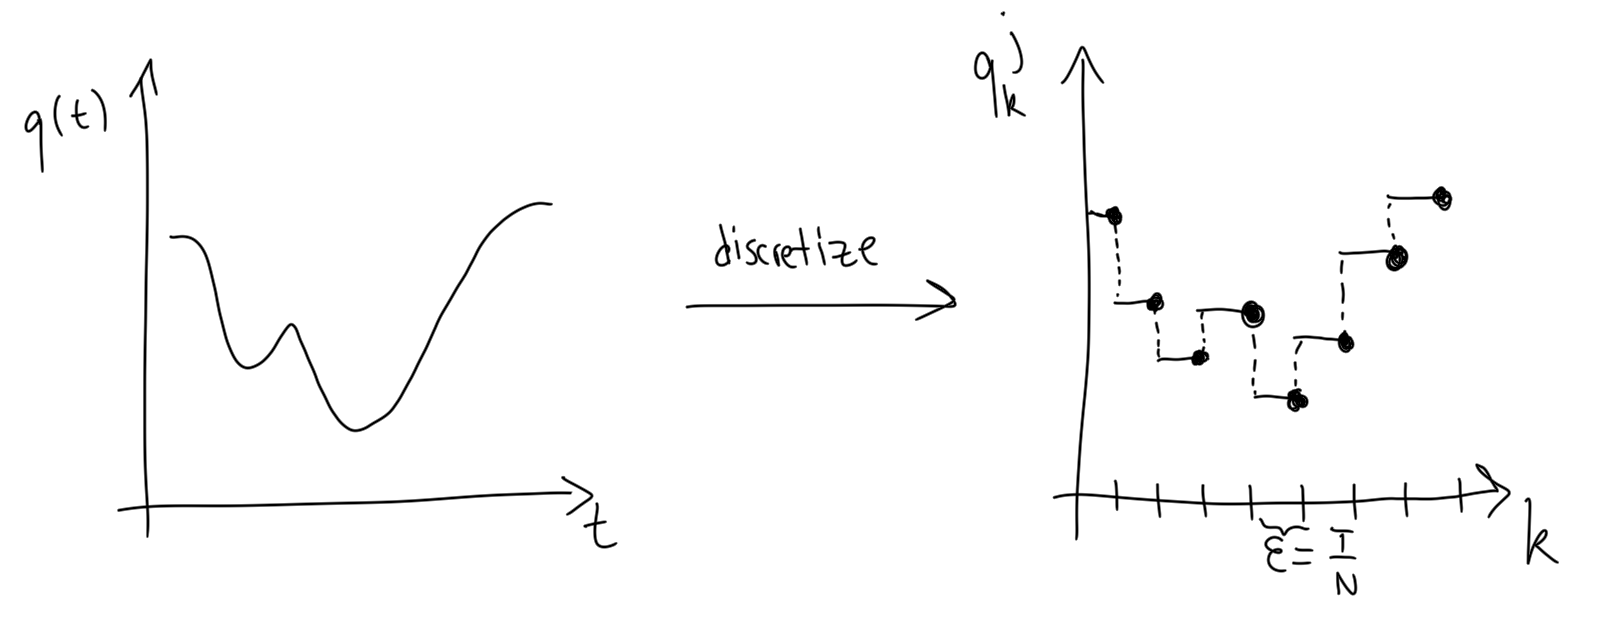
\includegraphics[width=4in]{images/discretize.png}
\end{figure}

\begin{equation}
U(q_i, q_f; T) = \left( \prod_{j, k} \int dq^j_k \int \frac{dp^j_k}{2\pi} \right) e^{i \sum_k (\sum_j p_k^j (q_{k+1}^j - q_k^j ) - \epsilon H)}
\end{equation}

\noindent Evaluate these very many integrals to get an answer dependent on $\epsilon = \frac{T}{N}$, since we discretized, take the limit as $\epsilon \rightarrow 0$ and deal with any encountered infinities.

\subsection*{Key Example}

\noindent Consider the classical Hamiltonian

\begin{equation}
H = \frac{p^2}{2 m} + V(q).
\end{equation}

\noindent Calculate the transition amplitude (\textbf{Exercise})

\begin{align}
U(q_i, q_f; T) &= \left( \prod_{j, k} \int dq^j_k \int \frac{dp^j_k}{2\pi} \right) e^{i \sum_k (\sum_j p_k^j (q_{k+1}^j - q_k^j ) - \epsilon H)} \\
&=  \left( \prod_{k} \int dq_k \int \frac{dp_k}{2\pi} \right) e^{i \sum_k (p_k (q_{k+1} - q_k ) - \epsilon (\frac{p_k^2}{2m} + V(q)) )} \\
&= \left( \prod_k \int dq_k \right) \sqrt{\frac{-im}{2\pi \epsilon}} e^{i \sum_k \frac{m}{2\epsilon} (q_{k+1} - q_k)^2 - \epsilon V\left(\frac{q_{k+1} + q_k}{2}\right)}.
\end{align}

\noindent We may also write this in the following notation, using the fact that the argument of the exponential is the discretized version of the action, now without the $p$-integral

\begin{equation}
\lim_{\epsilon \rightarrow 0} U(q_i, q_f; T) = \int \mathcal{D} q(t) e^{\mathcal{S}[q(t)]}
\end{equation}

\noindent Where the action is 

\begin{equation}
\mathcal{S}[q(t)] = \int^T_0 dt \,\, \left(\frac{m}{2} \sum_j (\dot{q}^j)^2 - V(q)\right).
\end{equation}

\noindent Note that if our system is a harmonic oscillator $V(q) = \frac{1}{2} m \omega^2 q^2$, we can do the full integral.

\subsection*{Path Integrals for Scalar Fields}

\noindent Recall the classical scalar field with Lagrangian density and Hamiltonian

\begin{align}
\mathcal{L} &= \frac{1}{2} (\partial_\mu \phi)^2 - V(\phi) \\
H &= \int d^3 x \,\, \left(\frac{1}{2} \pi^2(x) + \frac{1}{2} (\nabla \phi(x))^2 + V(\phi(x)) \right).
\end{align}

\noindent The path integral prescription for quantum scalar fields gives the transition amplitude, by blind application of the above, we conjecture that

\begin{equation}
\bra{\phi_b} e^{-i \hat{H} T} \ket{\phi_a} = \left( \int \mathcal{D} \phi \int \mathcal{D} \pi \right) e^{i \int^T_0 d^4x \, (\pi \dot{\phi} - H(\phi))}
\end{equation}

\noindent Where the boundary terms are $\phi(t=0, x) = \phi_a (\textbf{x})$ and $\phi(t=T, x) = \phi_b (\textbf{x})$. \\

\noindent As explained above, to make sense of this quantity, we must discretize, evaluate, and take the continuum limit as $\epsilon \rightarrow \infty$. When we discretize, note that we only discretize space, as discretizing time in this way will cause trouble with the conjugate momenta. \\

\noindent The field operators are discretized over a "grid" of points $x_j$ each of width $\epsilon$, such that

\begin{equation}
\phi(t, x) \,\,\, \rightarrow \,\,\, \phi(t, x_j) \equiv q^j (t).
\end{equation}

\noindent Then discretize the integral by turning it into a sum over the grid

\begin{equation}
\int d^3 x  \,\,\, \rightarrow \,\,\, \epsilon^3 \Sigma_{j \in \mathbb{Z}^3} .
\end{equation}

\noindent Next the derivative can be discretized via a finite difference. Note that there are more computationally efficient symmetric differences that can be used to discretize the derivative, but the finite difference works well for demonstration

\begin{equation}
\nabla_\mu \phi(x) \,\,\, \rightarrow  \,\,\, \frac{(\phi(x_j + \epsilon_\mu) - \phi(x_j))}{|\epsilon_\mu|}
\end{equation}

\noindent Where $\mu$ denotes the four directions in which to calculate the derivative

\begin{equation}
\epsilon_{\mu} = \epsilon \{ \left(\begin{smallmatrix}1\\0\\0\\0\end{smallmatrix}\right), \left(\begin{smallmatrix}0\\1\\0\\0\end{smallmatrix}\right), \left(\begin{smallmatrix}0\\0\\1\\0\end{smallmatrix}\right), \left(\begin{smallmatrix}0\\0\\0\\1\end{smallmatrix}\right) \}
\end{equation}.

\noindent Lastly, the potential just becomes evaluated at each $x_j$

\begin{equation}
V(\phi(x)) \,\,\, \rightarrow \,\,\, V(\phi(x_j)).
\end{equation}

\noindent Then the Lagrangian is discretized to a sum over a bunch of terms, but the only relevant term to the construction of the Hamiltonian is the time derivative of the field operator $\dot{\phi}$ (\textbf{Exercise})

\begin{equation}
L = \int d^3 x \, \mathcal{L} \rightarrow \epsilon^3 \sum_j \frac{1}{2} (\dot{\phi}_j)^2
\end{equation}

\noindent And the discretized conjugate momentum becomes

\begin{equation}
\pi^j = \frac{\partial L}{\partial \dot{q}^j} = \frac{\partial L}{\partial \dot{\phi}^j}  \,\,\, \rightarrow \,\,\, \epsilon^3 \dot{q}^j .
\end{equation}

\noindent Finally, we have the discretized Hamiltonian, where we display the $\epsilon$ terms to show that if we did not add the $\epsilon^3$ term to the discretized Lagrangian, we would be stuck with an extra $\epsilon^{-3}$ on the discretized Hamiltonian

\begin{equation}
H = \epsilon^3 \sum_j \epsilon^{-3} \pi_j^2 + \frac{1}{2} \left( \frac{q_{j+\epsilon^\mu}-q_j}{\epsilon} \right)^2 + V(q).
\end{equation}

\noindent In summary, the discretization of the scalar field gives us a nonrelativistic lattice system such that the discretized Hamiltonian is the sum of a kinetic energy term and a potential energy term. The second step is to evaluate the (nonrelativistic) path integral, and the third step is to take the continuum limit as $\epsilon \rightarrow 0$, which will later be re-branded as renormalization. \\

\noindent The most important case of the scalar field is the quadratic potential, which corresponds to the Klein-Gordon field (e.g., discretizing Klein-Gordon theory yields the quadratic potential below), is

\begin{equation}
V(q) = \frac{1}{2} q^T \textbf{A} q.
\end{equation}

\subsection*{Gaussian Integrals}

\noindent Consider the following integral 

\begin{equation}
I = \int_{-\infty}^\infty dx \,\, e^{-x^2} = \sqrt{\pi}.
\end{equation}

\noindent Proof:

\begin{align}
I &= \int_{-\infty}^\infty dx \,\, e^{-x^2} \\
I^2 &= \left(\int_{-\infty}^\infty dx \,\, e^{-x^2} \right) \left( \int_{-\infty}^\infty dy \,\, e^{-y^2}  \right) \\
I^2 &= \int_0^\infty r dr \, \int_0^{2\pi} d\theta \, e^{-r^2} \\
I^2 &= 2 \pi \int_0^\infty \frac{d}{dr} \left( -\frac{1}{2} e^{-r^2} \right) dr = \pi
\end{align} .

\noindent This is actually a special case of the more general forms of the Gaussian integral

\begin{align}
\int_{-\infty}^\infty dx \,\, e^{ -\frac{1}{2} a x^2 + b x } &= \sqrt{\frac{2\pi}{a}} e^{ \frac{b^2}{2a}  } \\
\int_{-\infty}^\infty dx \,\, e^{  i a x^2 + i b x } &= \sqrt{\frac{2\pi i}{a}} e^{ \frac{-i b^2}{2a}  } \\
\end{align}.

\noindent We will later need the moments generated by the Gaussian integral

\begin{align}
\langle x^n \rangle = \frac{\int_{-\infty}^\infty dx \,\, x^n e^{ -\frac{1}{2} a x^2}}{\int_{-\infty}^\infty dx \,\, e^{ -\frac{1}{2} a x^2}}.
\end{align}

\noindent Note that if $n$ is odd, then the moment is zero and we can write the exponent of $x$ as $2m$, where $m \in \mathbb{Z}$, and we have the relation (\textbf{Exercise})

\begin{equation}
\langle x^{2m} \rangle = \frac{(2m-1)!!}{a^m}.
\end{equation}

\noindent Note that the double factorial $(2m-1)!!$ represents the number of ways to join $2m$ points in pairs. -- "All science should in linear algebra or combinatorics." -- \\

\noindent Another closed form of this integral is in terms of derivatives is

\begin{align}
\langle x^{2m} \rangle &=  \left( \frac{d}{db} \right)^{2m} \left(  \frac{\int_{-\infty}^\infty dx \,\, e^{ -\frac{1}{2} a x^2 + b x }}{\int_{-\infty}^\infty dx \,\, e^{ -\frac{1}{2} a x^2 }} \right) \big|_{b=0} \\
\langle x^{2m} \rangle &= \left( \frac{d}{db} \right)^{2m} e^{\frac{b^2}{2a}} \big|_{b=0}.
\end{align}

\noindent To evaluate the maultivariable Gaussian integrals, where $x \in \mathbb{R}^n$, consider

\begin{equation}
I(\textbf{A}, B) = \int_{-\infty}^\infty dx_1 \dots \int_{-\infty}^\infty dx_n \,\, e^{-x^T \textbf{A} x + B^T x}
\end{equation}

\noindent Where $\textbf{A}$ is an $n \times n$ symmetric real matrix and $B$ is an $n \times 1$ real vector. Since $\textbf{A}$ is real, symmetric, it contains orthogonal $\textbf{O}$ and diagonal matrices $\textbf{D}$, such that $\textbf{O}^T \textbf{O} = \mathbb{I}$ and $\textbf{D}$ is diagonalized with the eignevalues of $\textbf{A}$.

\begin{equation}
\textbf{O}^T \textbf{D} \textbf{O} = \textbf{A}
\end{equation}

\noindent Assume that $B=0$ and define $y = \textbf{O} x$. Then

\begin{align}
I(\textbf{A}, B=0) &= \int_{-\infty}^\infty dy_1 \dots \int_{-\infty}^\infty dy_n \,\, e^{-y^T \textbf{D} y} \\
&= \prod_{j=1}^n \int_{-\infty}^\infty dy_j \,\, e^{-y_j^2 \lambda_j} \\
&= \prod_{j=1}^n \sqrt{\frac{\pi}{\lambda_j}} \\
I(\textbf{A}, B=0)&= \sqrt{\frac{\pi^n}{\text{det}(\textbf{A})}}.
\end{align}

\noindent The $B \ne 0$ case (\textbf{Exercise}) results in the following

\begin{equation}
I(\textbf{A},B) = \sqrt{\frac{\pi^n}{\text{det}(\textbf{A})}} e^{B^T \textbf{A}^{-1} B}.
\end{equation}